% Template for an EarthArXiv preprint of the manuscript.
% Includes the standard disclaimers and formatting that is required.
%
% This is the document structure. The actual content is written in:
% * abstract.tex: The abstract.
% * abstract-plain.tex: A plain language version of the abstract.
% * content.tex: The actual manuscript text (minus the abstract).
%
%%%%%%%%%%%%%%%%%%%%%%%%%%%%%%%%%%%%%%%%%%%%%%%%%%%%%%%%%%%%%%%%%%%%%%%%%%%%%%%
% Set a class and general configuration
\documentclass[onecolumn,10pt]{article}

%%%%%%%%%%%%%%%%%%%%%%%%%%%%%%%%%%%%%%%%%%%%%%%%%%%%%%%%%%%%%%%%%%%%%%%%%%%%%%%
% Set variables with the title, authors, etc.
\newcommand{\Title}{The long version of the paper title}
\newcommand{\TitleShort}{A short title}

\newcommand{\Year}{2023}
\newcommand{\SubmittedOn}{2023/02/28}
\newcommand{\PublishedOn}{2023/02/28}

\newcommand{\AuthorShort}{Uieda \textit{et al.}}
\newcommand{\Authors}{%
  Leonardo Uieda\textsuperscript{1},
  Santiago R. Soler\textsuperscript{2}
}
\newcommand{\Email}{contact-email@university.org}
\newcommand{\Corresponding}{%
  Corresponding author: Leonardo Uieda <\href{mailto:\Email}{\Email}>
}
\newcommand{\Affiliations}{%
  \textsuperscript{1} Universidade de São Paulo, Brazil;
  \textsuperscript{2} University of British Columbia, Canada;
}

\newcommand{\Journal}{Geochemistry, Geophysics, Geosystems}
\newcommand{\JournalDOI}{YYYYY/YYYYYYY}
\newcommand{\PreprintDOI}{XXXXX/XXXXXXX}
\newcommand{\ArchiveDOI}{DOI_FOR_THE_REPO_ARCHIVE}
\newcommand{\GitHubRepository}{compgeolab/paper-template}

\newcommand{\Keywords}{%
  keyword1; keyword2; keyword3;
}

%%%%%%%%%%%%%%%%%%%%%%%%%%%%%%%%%%%%%%%%%%%%%%%%%%%%%%%%%%%%%%%%%%%%%%%%%%%%%%%
% Import the required packages
\usepackage[utf8]{inputenc}
\usepackage[TU]{fontenc}
\usepackage[english]{babel}
\usepackage{amsmath}
\usepackage{amssymb}
\usepackage{graphicx}
\usepackage{hyperref}
\usepackage{fancyhdr}
\usepackage{orcidlink}
\usepackage{geometry}
\usepackage{booktabs}
\usepackage{microtype}
\usepackage{siunitx}
% To customize the title page
\usepackage{titling}
% For adding multiple authors
\usepackage{authblk}
% improved urls with proper hyphenation
\usepackage{xurl}
% Tweak the look of captions
\usepackage{caption}
% To control the style of section titles
\usepackage{titlesec}
% Import natbib and doi packages
\usepackage[round,authoryear,sort]{natbib}
% show dois as links on references
\usepackage{doi}
% Remove extra space between references
\usepackage{natbibspacing}
% Use a different font
\usepackage[scaled=1.1]{notomath}
% Icons and fonts (requires using xelatex or luatex)
\usepackage{fontawesome5}
\usepackage{academicons}
% Control the font size
\usepackage{anyfontsize}
\usepackage{setspace}
% To get the number of pages in the document
\usepackage{lastpage}
\usepackage{lipsum}
\usepackage{ragged2e}
\usepackage{mdframed}
% To define custom environments
\usepackage{environ}
% To control hyphenation for individual blocks of text
\usepackage{hyphenat}


%%%%%%%%%%%%%%%%%%%%%%%%%%%%%%%%%%%%%%%%%%%%%%%%%%%%%%%%%%%%%%%%%%%%%%%%%%%%%%%
% Configuration of the document

\geometry{%
  left=25mm,
  right=25mm,
  top=18mm,
  bottom=15mm,
  headsep=0mm,
  headheight=0mm,
  footskip=7mm,
  includehead=true,
  includefoot=true
}

% Control line and table row spacing
\onehalfspacing
\renewcommand{\arraystretch}{1.5}

% Set the spacing between bibliography entries (requires natbib)
\setlength{\bibsep}{0pt}

% Custom colors
\definecolor{darkgray}{gray}{0.4}
\definecolor{mediumgray}{gray}{0.5}
\definecolor{lightgray}{gray}{0.9}
\definecolor{mediumblue}{HTML}{2060c2}
\definecolor{lightblue}{HTML}{f7faff}

% Configure captions
\captionsetup[table]{position=below,skip=0pt}
\captionsetup{labelfont=bf,font={small,color=darkgray},skip=10pt}

% Make urls use the same font as every other text
\urlstyle{same}

% Configure hyperref and add PDF metadata
\hypersetup{
    colorlinks,
    allcolors=mediumblue,
    pdftitle={\Title},
    pdfauthor={\AuthorShort},
    breaklinks=true,
}

% Configure header and footer
% Inspired by LaPreprint: https://github.com/roaldarbol/LaPreprint
\newcommand{\Separator}{\hspace{3pt}|\hspace{3pt}}
\newcommand{\FooterFont}{\footnotesize\color{mediumgray}}
\pagestyle{fancy}
\fancyhf{}
\lfoot{%
  \FooterFont{}
  \AuthorShort{} (\Year)
  \Separator{}
  \TitleShort
}
\rfoot{%
  \FooterFont{}
  EarthArXiv
  \Separator{}
  \thepage\space of\space \pageref*{LastPage}
}
\renewcommand{\headrulewidth}{0pt}
\renewcommand{\footrulewidth}{1pt}
\preto{\footrule}{\color{lightgray}}
\fancypagestyle{plain}{%
  \fancyhf{}
  \lfoot{%
    \FooterFont{}
    \faCreativeCommons\faCreativeCommonsBy
    \Separator{}
    \textcopyright{} \Year{} The Authors
  }
  \rfoot{%
    \FooterFont{}
    doi:\href{https://doi.org/\PreprintDOI}{\PreprintDOI}
    \Separator{}
    EarthArXiv
    \Separator{}
    \thepage\space of\space \pageref*{LastPage}
  }
}

% Define fancy text boxes
\NewEnviron{summarybox}{%
  \mdfdefinestyle{summarybox_}{%
    leftline=true,
    rightline=false,
    topline=false,
    bottomline=false,
    linewidth=2pt,
    linecolor=mediumblue,
    backgroundcolor=lightblue,
    innertopmargin=12pt,
    innerbottommargin=12pt,
    innerleftmargin=12pt,
    innerrightmargin=12pt,
    skipbelow=5pt,
    skipabove=5pt,
  }
  \newmdenv[style=summarybox_]{summarybox_}
  \begin{summarybox_}
    \footnotesize
    \BODY
  \end{summarybox_}
}

%%%%%%%%%%%%%%%%%%%%%%%%%%%%%%%%%%%%%%%%%%%%%%%%%%%%%%%%%%%%%%%%%%%%%%%%%%%%%%%
\begin{document}

\thispagestyle{plain}
\begin{FlushLeft}
  \begin{spacing}{2}
    {\LARGE\bfseries \Title}
  \end{spacing}
  {\color{lightgray}\hrule height 1.5pt}
  \vspace{0.3cm}
  \Authors
  \\[0.2cm]
  {\footnotesize \Affiliations}
  \newline
  {\footnotesize \Corresponding}
  \\[0.2cm]
  {\footnotesize
    Received in original form on \SubmittedOn.
    %Published in final form on \PublishedOn.
  }
\end{FlushLeft}

\begin{summarybox}
  \noindent
  \textbf{Disclaimer:}
  %This is a non-peer reviewed preprint of an article submitted for publication
  %in \textit{\Journal{}}. It is available from EarthArXiv at
  %\url{https://doi.org/\PreprintDOI}.
  %%%%%%%%%%%%%%%%%%%%%%%%%%%%%%%%%%%%%%%%%%%%%%%%%%%%%%%%%%%%%%%%%%%%%%%%%%%%%
  % Comment the above and uncomment below after publication in a journal
  %%%%%%%%%%%%%%%%%%%%%%%%%%%%%%%%%%%%%%%%%%%%%%%%%%%%%%%%%%%%%%%%%%%%%%%%%%%%%
  This is a peer-reviewed author-produced postprint of the article
  ``\AuthorShort{} (\Year). \Title. \textit{\Journal}.
  doi:\href{https://doi.org/\JournalDOI}{\JournalDOI}''.
  The postprint is available from EarthArXiv at
  \url{https://doi.org/\PreprintDOI}.
  %%%%%%%%%%%%%%%%%%%%%%%%%%%%%%%%%%%%%%%%%%%%%%%%%%%%%%%%%%%%%%%%%%%%%%%%%%%%%
  \\[0.25cm]
  \noindent
  \textbf{Open research:}
  The source code used to generate all of the results presented in this
  research can be freely accessed and reused under the terms of an open license.
  You can find it at \url{https://doi.org/\ArchiveDOI} and
  \url{https://github.com/\GitHubRepository}.
  \\[0.25cm]
  \noindent
  \textbf{Keywords:} \Keywords{}
  \\[0.25cm]
  \noindent
  \textbf{\textcopyright{} \Year{} The Authors.}
  Available under the \href{https://creativecommons.org/licenses/by/4.0/}{Creative Commons Attribution 4.0 International License}
  \faCreativeCommons\faCreativeCommonsBy{}.
\end{summarybox}

\section*{\normalsize Plain language summary}
\begingroup
  \setstretch{1.1} \small \input{abstract-plain} \par
\endgroup

\section*{\normalsize Abstract}
\begingroup
  \setstretch{1.1} \small %Custom abstract
\singlespacing
\selectlanguage{english}
\section*{\centering{\footnotesize{ABSTRACT}}}
    \begin{adjustwidth}{18pt}{38pt}
            \setstretch{1.0}{
            \footnotesize
            % Paleomagnetic data are usually obtained from whole cylindric samples, where the signal results from the sum of magnetic moments from hundreds of thousands to millions of magnetic particles within the sample volume. 
            % This usually includes both stable and unstable remanence carriers.
            % Recently, magnetic microscopy techniques allowed the investigation of individual grains by directly imaging their magnetic field. 
            % However, the determination of the magnetic moments of individual grains is hindered by the intrinsic ambiguity in the inversion of potential field data, as well as by the large number of grains found in any one microscopy image. In our previous work,
            % we presented a fast, semi-automated algorithm capable of estimating the position and magnetization of each ferromagnetic (l.s) source using only the magnetic microscopy data. 
            % Our algorithm works in three steps: (i) we first apply image processing techniques to identify and isolate data window boundaries for each source; (ii) with these window boundaries, the position of the sources is estimated using Euler deconvolution; and finally (iii) using the  position information, the algorithm is able to estimate the magnetic dipole moment direction and intensity for each source through an overdetermined linear inverse problem using a dipolar approximation. 
            % The method does not require any type of additional information about the sample or the sources. Tests with simple synthetic data show the high effectiveness of the methodology for recovering the position and magnetic information for both dipolar and non-dipolar sources. 
            % More complex synthetic data including over 100 different magnetic particles were devised to emulate real rock data. 
            % Results obtained on these data also show the feasibility and robustness of the algorithm to semi-automatically estimate the position and magnetic moment of a large number of particles. 
            % This is further confirmed through an application to real data in which we are able to retrieve the expected bimodal isothermal remanent directions that were induced in the sample. 
            % Given its semi-automatic nature, its low processing cost, and the possibility of simultaneous inversion of the magnetic moment of a great number of magnetic particles, the methodology here proposed is a step forward in enabling paleomagnetic applications of magnetic microscopy.

        In the context of paleomagnetism, we face the challenge of obtaining crucial information about magnetic sources present in rock samples using non-invasive techniques without the need for costly and limiting additional methods. In our previous work, we proposed an innovative approach aimed at obtaining a priori information about magnetic sources based solely on data generated by magnetic microscopy. Our approach begins with the identification of the region where the signal from magnetic particles is present in the rock sample. Using an edge detection algorithm, we isolate these areas of interest, creating "slices" of data. We then apply the Euler deconvolution (ED) technique to these data windows to estimate the three-dimensional position of the magnetic particles, assuming they behave as point dipolar sources. The results of our synthetic tests demonstrate the effectiveness of our methodology. We tested point dipolar sources with varying magnetization in terms of direction, intensity, and depth. The algorithm not only identified all the source windows, including the weakest ones, but also produced minimal differences between the modeled position and the position estimated by ED. Furthermore, we conducted tests with complex magnetization sources and the Euler algorithm continued to work effectively even for non-dipolar fields. The magnetic moment recovery was also very effective for dipolar and non-dipolar synthetic sources, which enabled further tests with real data samples (speleothems). In the latter, the magnetic directions estimated were also coherent with the induce isothermal remanent magnetization. However, some limitations with our approach were detected and this report mainly represents an attempt to tackle and solve these limitations, and also strategies to improve the proposed methodology.
            
            
        }
        \end{adjustwidth}


% \newpage
% \selectlanguage{brazil}
% \section*{\centering{\footnotesize{RESUMO}}}
% 	\begin{adjustwidth}{18pt}{38pt}
% 	    \setstretch{1.0}{
%      \footnotesize
%      Os dados paleomagnéticos são geralmente obtidos a partir de amostras cilíndricas completas, onde o sinal resulta da soma dos momentos magnéticos de centenas de milhares a milhões de partículas magnéticas dentro do volume da amostra. Isso normalmente inclui portadores de remanescência estáveis e instáveis. Recentemente, as técnicas de microscopia magnética permitiram a investigação de grãos individuais através da imagem direta de seus campos magnéticos. No entanto, a determinação dos momentos magnéticos de grãos individuais é dificultada pela ambiguidade intrínseca na inversão dos dados do campo potencial, bem como pelo grande número de grãos encontrados em qualquer imagem de microscopia. Apresentamos um algoritmo rápido e semi-automatizado capaz de estimar a posição e a magnetização de cada fonte ferromagnética (l.s) usando apenas os dados de microscopia magnética. Nosso algoritmo funciona em três etapas: (i) aplicamos técnicas de processamento de imagem para identificar e isolar as fronteiras das janelas de dados para cada fonte; (ii) com essas fronteiras de janelas, a posição das fontes é estimada usando a deconvolução de Euler; e, finalmente, (iii) usando as informações de posição, o algoritmo é capaz de estimar a direção e intensidade do momento dipolar magnético para cada fonte através de um problema inverso linear sobredeterminado usando uma aproximação dipolar. O método não requer nenhum tipo de informação adicional sobre a amostra ou as fontes. Foram realizados testes de sensibilidade para estimar a estabilidade de nossa rotina em relação à profundidade das partículas, razão sinal-ruído e não dipolaridade das fontes. Testes com dados sintéticos simples mostram a alta efetividade da metodologia na recuperação das informações de posição e magnetismo tanto para fontes dipolares quanto não dipolares. Dados sintéticos mais complexos, incluindo mais de 100 partículas magnéticas diferentes, foram criados para emular dados reais de rochas. Os resultados obtidos com esses dados também demonstram a viabilidade e robustez do algoritmo para estimar semi-automaticamente a posição e o momento magnético de um grande número de partículas. Isso é confirmado por meio de uma aplicação a dados reais em que conseguimos recuperar as direções esperadas de remanescência isotérmica bimodal que foram induzidas na amostra. Dada a sua natureza semi-automática, baixo custo de processamento e possibilidade de inversão simultânea do momento magnético de um grande número de partículas magnéticas, a metodologia aqui proposta representa um avanço na capacidade de aplicar a microscopia magnética em estudos paleomagnéticos.
%         }
% 	 \end{adjustwidth}
\selectlanguage{english}
\doublespacing
\newpage \par
\endgroup

\section{Introduction}

This is the introduction. Here's a text citation of \citet{OliveiraJr2015}
and a another version that is sometimes used \citep{OliveiraJr2015}.
The rest is gibberish text.




%%%%%%%%%%%%%%%%%%%%%%%%%%%%%%%%%%%%%%%%%%%%%%%%%%%%%%%%%%%%%%%%%%%%%%%%%%%%%%%
\section{Methodology}

Our algorithm for estimating the source's positioning based on Euler deconvolution revealed that stronger sources may influence the estimated positions of nearby weaker ones. Therefore, it becomes imperative to consider the interplay among magnetic sources to accurately estimate their magnetic parameters and position. Understanding how these magnetic sources interact with each other is crucial for refining our estimation process and ensuring robust results in magnetic parameter estimation.


\subsection{Magnetic inversion: interfering sources}
    
In this study, our objective is to explore three distinct methods for handling interfering sources during inversion. The first approach involves employing the interactive Euler deconvolution method, where interference from other sources is systematically removed in each window. The second method considers interference using the $b_z$ vector. The inversion is performed on the entire set of particles. Lastly, we explore a similar approach as the second method, but applied to the first derivative of $b_z$.


\subsubsection{Iteractive Euler deconvolution}

Our algorithm for estimating the source's positioning based on Euler deconvolution revealed that stronger sources may influence the estimated positions of nearby weaker ones. To address this, we propose a refined algorithm with the following steps:

\begin{enumerate}
  \item \textbf{Automatic Source Detection:} Utilizing blob detection on the total gradient amplitude (TGA), the algorithm segregates sources in descending order of magnitude. This enables the application of Euler deconvolution to obtain an initial position estimation.
  
  \item \textbf{Calculation of Theoretical Magnetic Signals:} The theoretical magnetic signals associated with these sources are computed using a simple dipolar forward model.
  
  \item \textbf{Signal Removal:} The magnetic signal attributed to the strongest source is then removed from the original dataset.
  
  \item \textbf{Enhanced Estimation:} The refined dataset is subsequently employed for the analysis of weaker magnetic sources, leading to an improved positioning estimation compared to the previous step.
\end{enumerate}

This step-by-step procedure is designed to mitigate the impact of stronger sources, thereby enhancing the precision of subsequent inversion analyses.



\subsubsection{Vertical component magnetic field}
A way to improve the inversion results is to perform the magnetic moment estimation of all L sources identified at the same time: 

\begin{equation}
\footnotesize
\label{eq_dipole_bz_all}
\dfrac{\mu_0}{4\pi}
{\begin{bmatrix}
\dfrac{\partial^2}{\partial z \partial x} \dfrac{1}{r_{1,1}}
& \dfrac{\partial^2}{\partial z \partial y} \dfrac{1}{r_{1,1}}
& \dfrac{\partial^2}{\partial z \partial z} \dfrac{1}{r_{1,1}}
& \hdots
& \dfrac{\partial^2}{\partial z \partial x} \dfrac{1}{r_{1,L}}
& \dfrac{\partial^2}{\partial z \partial y} \dfrac{1}{r_{1,L}}
& \dfrac{\partial^2}{\partial z \partial z} \dfrac{1}{r_{1,L}} \\
\\

& 
& 
& \vdots
& 
& 
&  \\
\\
\dfrac{\partial^2}{\partial z \partial x} \dfrac{1}{r_{N,1}}
& \dfrac{\partial^2}{\partial z \partial y} \dfrac{1}{r_{N,1}}
& \dfrac{\partial^2}{\partial z \partial z} \dfrac{1}{r_{N,1}}
& \hdots
& \dfrac{\partial^2}{\partial z \partial x} \dfrac{1}{r_{N,L}}
& \dfrac{\partial^2}{\partial z \partial y} \dfrac{1}{r_{N,L}}
& \dfrac{\partial^2}{\partial z \partial z} \dfrac{1}{r_{N,L}} \\
\end{bmatrix}}_{N x L}
{\begin{bmatrix}
{m_x}_1 \\ {m_y}_1 \\ {m_z}_1 \\ \vdots \\{m_x}_L \\ {m_y}_L \\ {m_z}_L \\
\end{bmatrix}}_{L x 1}
=
{\begin{bmatrix}
{bz}_1 \\ {bz}_2 \\ {bz}_3 \\ \vdots \\{bz}_N 
\end{bmatrix}}_{N x 1}.
\end{equation} \bigskip

In which $r_{i,j} = \sqrt{(x_i - {x_c}_j)^2 + (y_i - {y_c}_j)^2 + (z_i - {z_c}_j)^2}$ is the Cartesian distance between the i-th, $i=1, 2, \hdots N$, observation point $b_z (x_i, y_i, z_i)$ and the j-th, $j=1, 2, \hdots L$, point source $({x_c}_j, {y_c}_j, {z_c}_j)$ and $\mu_0$ is the vacuum magnetic permeability. While the three second-order derivatives in Equation~\ref{eq_dipole_bz_all} are:

\begin{equation}
\footnotesize
\begin{aligned}
\dfrac{\partial^2}{\partial z \partial x} \dfrac{1}{r_{i,j}} &=
\dfrac{3(z_i - {z_c}_j)(x_i - {x_c}_j)}{{r_{i,j}}^5}\ ,
\\
\dfrac{\partial^2}{\partial z \partial y} \dfrac{1}{r_{i,j}} &=
\dfrac{3(z_i - {z_c}_j)(y_i - {y_c}_j)}{{r_{i,j}}^5}\ ,
\\
\dfrac{\partial^2}{\partial z \partial z} \dfrac{1}{r_{i,j}} &=
\dfrac{3(z_i - {z_c}_j)^2}{{r_{i,j}}^5} - \dfrac{1}{{r_{i,j}}^3}\ .
\end{aligned}
\end{equation}   \bigskip

Therefore, taking into account all their mutual signal interference in the N observed data further causes the trade-off between accuracy and running time.




\subsubsection{First derivative of vertical component magnetic field}

The other way to improve the inversion process is by using the first derivative of $b_z$. The latter works  akin to a high-pass filter, thus, reducing the likelihood of the stronger source's long-wavelength signal causing too much interference with weaker ones. We can use the $\frac{b_z}{\partial z}$ by deriving both sides of Equation~\ref{eq_dipole_bz_all} by $z$:

\begin{equation}
\footnotesize
\label{eq_dipole_bz_z_deriv}
\dfrac{\mu_0}{4\pi}
\scriptsize{\begin{bmatrix}
\dfrac{\partial^2}{\partial z \partial x \partial z} \dfrac{1}{r_{1,1}}
& \dfrac{\partial^2}{\partial z \partial y \partial z} \dfrac{1}{r_{1,1}}
& \dfrac{\partial^2}{\partial z \partial z \partial z} \dfrac{1}{r_{1,1}}
& \hdots
& \dfrac{\partial^2}{\partial z \partial x \partial z} \dfrac{1}{r_{1,L}}
& \dfrac{\partial^2}{\partial z \partial y \partial z} \dfrac{1}{r_{1,L}}
& \dfrac{\partial^2}{\partial z \partial z \partial z} \dfrac{1}{r_{1,L}} \\
\\

& 
& 
& \vdots
& 
& 
&  \\
\\
\dfrac{\partial^2}{\partial z \partial x \partial z} \dfrac{1}{r_{N,1}}
& \dfrac{\partial^2}{\partial z \partial y \partial z} \dfrac{1}{r_{N,1}}
& \dfrac{\partial^2}{\partial z \partial z \partial z} \dfrac{1}{r_{N,1}}
& \hdots
& \dfrac{\partial^2}{\partial z \partial x \partial z} \dfrac{1}{r_{N,L}}
& \dfrac{\partial^2}{\partial z \partial y \partial z} \dfrac{1}{r_{N,L}}
& \dfrac{\partial^2}{\partial z \partial z \partial z} \dfrac{1}{r_{N,L}} \\
\end{bmatrix}}_{N x L}
{\begin{bmatrix}
{m_x}_1 \\ {m_y}_1 \\ {m_z}_1 \\ \vdots \\{m_x}_L \\ {m_y}_L \\ {m_z}_L \\
\end{bmatrix}}_{L x 1}
=
{\begin{bmatrix}
\frac{{bz}_1}{ \partial z} \\ \frac{{bz}_2}{ \partial z} \\ \frac{{bz}_3}{ \partial z} \\ \vdots \\\frac{{bz}_N}{ \partial z}
\end{bmatrix}}_{N x 1}.
\end{equation} \bigskip

Where the three third-order derivatives in Equation~\ref{eq_dipole_bz_z_deriv} are given by

\begin{equation}
\footnotesize
\begin{aligned}
\dfrac{\partial^2}{\partial z \partial x \partial z} \dfrac{1}{r_{i,j}} &=
\dfrac{3(x_i - {x_c}_j)}{{r_{i,j}}^5} - \dfrac{15(x_i - {x_c}_j)(z_i - {z_c}_j)^2}{{r_{i,j}}^7}\ ,
\\
\dfrac{\partial^2}{\partial z \partial y \partial z} \dfrac{1}{r_{i,j}} &=
\dfrac{3(y_i - {y_c}_j)}{{r_{i,j}}^5} - \dfrac{15(y_i - {y_c}_j)(z_i - {z_c}_j)^2}{{r_{i,j}}^7}\ ,
\\
\dfrac{\partial^2}{\partial z \partial z \partial z} \dfrac{1}{r_{i,j}} &=
\dfrac{9(z_i - {z_c}_j)}{{r_{i,j}}^5} - \dfrac{15(z_i - {z_c}_j)^3}{{r_{i,j}}^7}\ .
\end{aligned}
\end{equation}   \bigskip



%%%%%%%%%%%%%%%%%%%%%%%%%%%%%%%%%%%%%%%%%%%%%%%%%%%%%%%%%%%%%%%%%%%%%%%%%%%%%%%
\section{Results}


%\begin{figure}[tb]
%\centering
%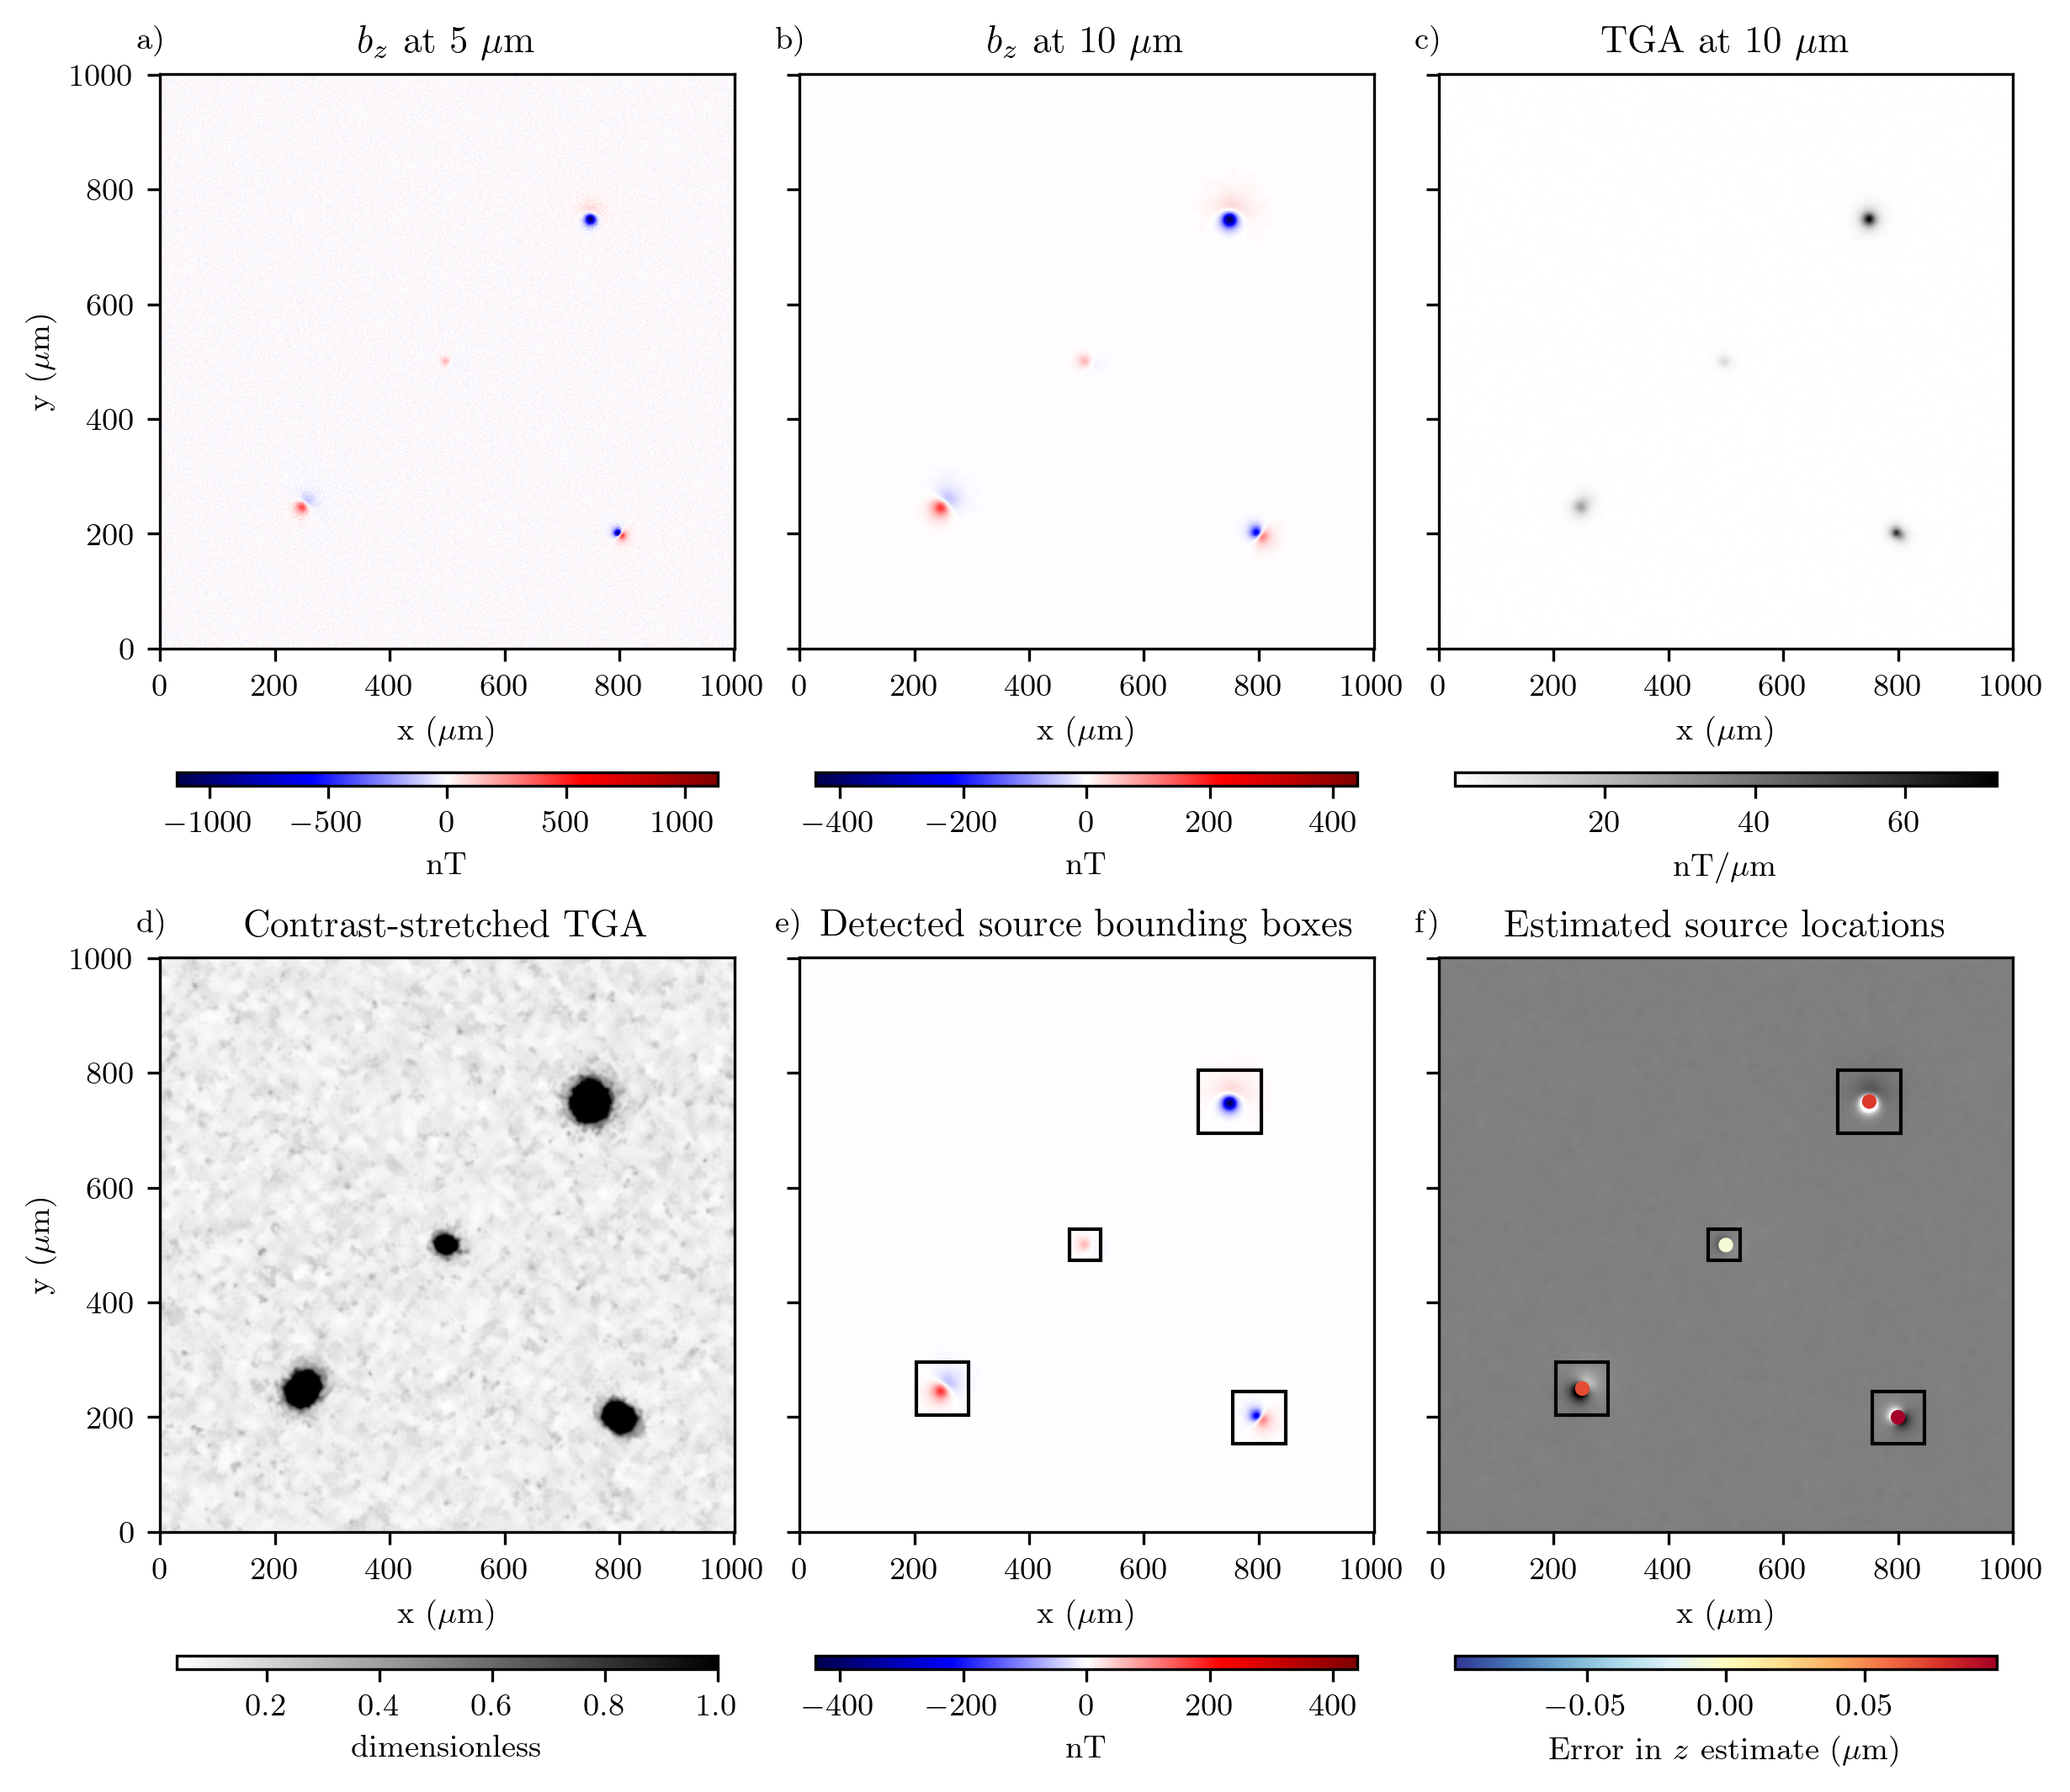
\includegraphics[width=1\linewidth]{figures/simple-synthetic-data.png}
%\caption{
  %\lipsum[1]
%}
%\label{fig_synthetic_simple_data}
%\end{figure}



%%%%%%%%%%%%%%%%%%%%%%%%%%%%%%%%%%%%%%%%%%%%%%%%%%%%%%%%%%%%%%%%%%%%%%%%%%%%%%%
\section{Discussions}


%%%%%%%%%%%%%%%%%%%%%%%%%%%%%%%%%%%%%%%%%%%%%%%%%%%%%%%%%%%%%%%%%%%%%%%%%%%%%%%
\section{Conclusion}



%%%%%%%%%%%%%%%%%%%%%%%%%%%%%%%%%%%%%%%%%%%%%%%%%%%%%%%%%%%%%%%%%%%%%%%%%%%%%%%
\section{Open research}

The Python source code used to produce all results and figures presented here
is available at \url{https://github.com/\GitHubRepository} and
\url{https://doi.org/\ArchiveDOI} under the MIT open-source license.

Here we should cite all of the main software used, like Jupyter, numpy, scipy,
matplotlib, Fatiando, etc.

Cite any data sources as well.



%%%%%%%%%%%%%%%%%%%%%%%%%%%%%%%%%%%%%%%%%%%%%%%%%%%%%%%%%%%%%%%%%%%%%%%%%%%%%%%
\section{Acknowledgements}

We are indebted to the developers and maintainers of the open-source software
without which this work would not have been possible.
Acknowledge any non-author contributors to this study.
Statement about funding.

% Thank the editors and reviewers after review.


\bibliographystyle{apalike-doi}
\bibliography{references}

\end{document}
